\documentclass[10pt,bezier]{article}

\usepackage{graphicx}
\usepackage{amsmath, bm, amssymb}
\interdisplaylinepenalty=2500
\usepackage{color}
\usepackage{caption}

\usepackage{enumerate}
\usepackage[colorlinks,urlcolor=blue,citecolor=blue,linkcolor=blue]{hyperref}
%\usepackage[short]{optidef}
\usepackage{blindtext}
\usepackage{mathtools}
\usepackage{mathptmx}
\usepackage{makeidx}
\usepackage{latexsym}
\usepackage{epsfig}
\usepackage{url}
\usepackage{etoolbox}
\usepackage{float}
\usepackage{bbding}
\usepackage{lineno,xcolor}
\usepackage{xcolor}
\usepackage{empheq}
%\usepackage[thinlines]{easytable}
\usepackage{amsfonts}
\usepackage{array}
\usepackage{booktabs}
\usepackage{multirow}
%\usepackage{algorithm}
\usepackage[ruled,vlined]{algorithm2e}
\usepackage[letterpaper, margin=1in]{geometry}

\begin{document}

%------------------------------------------------------------------------------------------------------------------------------------
%------------------------------------------------------------------------------------------------------------------------------------
\section*{Examples for Walmart Interview}\label{Title}
Author: Daniel A. Zuniga Vazquez\\

\noindent Written in \textbf{LaTeX} and coded as specified in:\\
- {\color{blue}\textbf{C++}} and {\color{blue}\textbf{C\#}} using Visual Studio\\
- {\color{blue}\textbf{Java}} using Eclipse\\
- {\color{blue}\textbf{Python}} using Anaconda with Jupyter Notebook
\tableofcontents

\newpage
%------------------------------------------------------------------------------------------------------------------------------------
%------------------------------------------------------------------------------------------------------------------------------------
\section{Vehicle Routing Problem (VRP)}\label{section1}

\subsection{Two Index Vehicle Routing Formulation}\label{section1.1}
The following vehicle routing example is coded in {\color{blue}\textbf{C++}}, {\color{blue}\textbf{C\#}}, {\color{blue}\textbf{Python}} and {\color{blue}\textbf{Java}}:\\

\noindent Sets and indices
\begin{itemize}
  \item $D$:~Set of destinations, indexed by $i$, $j$.
\end{itemize}
Parameters
\begin{itemize}
    \item $c_{ij}$:~ Vehicle routing cost from vertex $i$ to vertex $j$.
    \item $K$:~Number of vehicles.
    \item $MAX$:~Maximum number of destinations a vehicle can be routed to.
\end{itemize}
Variables
\begin{itemize}
  \item $x_{ij}$:~Binary variables that is 1 if a vehicle is routed from destination $i$ to destination $j$ and 0 otherwise.
  \item $y_i$:~Integer variable that denotes the destination $i$ position in the vehicle routing.
\end{itemize}

\noindent The vehicle routing formulation is presented as follows:

\begin{subequations}
    \begin{align}
    \min_{\pmb{x},\pmb{y}}~& \sum_{i \in D} \sum_{j \in D} c_{ij} x_{ij}  \tag{Minimize total cost}\\
    \text{s.t. } & \sum_{i \in D} x_{ij} = 1,~ \forall j \in D \setminus \{0\}: j \neq i \tag{1.1a - Only one vehicle can enter a destination}\\
                 & \sum_{j \in D} x_{ij} = 1,~ \forall i \in D \setminus \{0\}: i \neq j \tag{1.1b - Only one vehicle can leave a destination}\\
                 & \sum_{i \in D \setminus \{0\}} x_{i0} = K \tag{1.1c - Number of vehicles leaving the depot at destination 0}\\
                 & \sum_{j \in D \setminus \{0\}} x_{0j} = K \tag{1.1d - Number of vehicles entering the depot at destination 0}\\
                 & y_i - y_j + MAX~x_{ij} \leq MAX -1,~\forall i, j \in D \setminus \{0\} : i \neq j \tag{1.1e - Subtour elimination (Miller-Tucker-Zemlin)}\\
                 & x_{i,j} \in \{0,1\}, y_i \in \mathbb{Z},~\forall i \in I, \forall j \in J  \tag{1.1f - Domain}
    \end{align}
\end{subequations}

\newpage
%------------------------------------------------------------------------------------------------------------------------------------
%------------------------------------------------------------------------------------------------------------------------------------
\section{Facility Location}\label{section2}

\subsection{Capacitated Facility Location}\label{section2.1}
The following facility location example is coded in {\color{blue}\textbf{C++}}, {\color{blue}\textbf{C\#}}, {\color{blue}\textbf{Python}} and {\color{blue}\textbf{Java}}:\\

\noindent Sets and indices
\begin{itemize}
  \item $I$:~Set of facilities, indexed by $i$.
  \item $J$:~Set of customers, indexed by $j$.
\end{itemize}
Parameters
\begin{itemize}
    \item $c_{ij}$:~ Cost of facility $i$ to supply to customer $j$.
    \item $d_j$:~Demand of customer $j$.
    \item $f_i$:~Cost of adding facility $i$.
    \item $u_i$:~Capacity of facility $i$.
\end{itemize}
Variables
\begin{itemize}
  \item $x_i$:~Binary variables that is 1 if facility $i$ is assigned and 0 otherwise.
  \item $y_{ij}$:~Fraction of demand supplied from facility $i$ to customer $j$.
\end{itemize}

\noindent The capacitated facility location formulation is presented as follows:

\begin{subequations}
    \begin{align}
    \min_{\pmb{x},\pmb{y}}~& \sum_{i \in I} \sum_{ j \in J} c_{ij} d_j y_{ij} + \sum_{i \in I} f_i x_i  \tag{Minimize total cost}\\
    \text{s.t. } & \sum_{i \in I} y_{ij} = 1,~\forall j \in J \tag{2.1a - Satisfied fraction of demand}\\
                 & \sum_{j \in J} d_j y_{ij} \leq u_i x_i,~\forall i \in I \tag{2.1b - Facility capacity}\\
                 & y_{ij} \leq 0, x_i \in \{0,1\},~\forall i \in I, \forall j \in J  \tag{2.1c - Domain}
    \end{align}
\end{subequations}

\newpage
\subsection{Uncapacitated Facility Location}\label{section2.2}
The following facility location example is coded in {\color{blue}\textbf{C++}}, {\color{blue}\textbf{C\#}}, {\color{blue}\textbf{Python}} and {\color{blue}\textbf{Java}}:\\

\noindent Sets and indices
\begin{itemize}
  \item $I$:~Set of facilities, indexed by $i$.
  \item $J$:~Set of customers, indexed by $j$.
\end{itemize}
Parameters
\begin{itemize}
    \item $c_{ij}$:~ Cost of facility $i$ to supply to customer $j$.
    \item $d_j$:~Demand of customer $j$.
    \item $f_i$:~Cost of adding facility $i$.
    \item $M$:~Big M, i.e., sufficiently big number.
\end{itemize}
Variables
\begin{itemize}
  \item $x_i$:~Binary variables that is 1 if facility $i$ is assigned and 0 otherwise.
  \item $y_{ij}$:~Fraction of demand supplied from facility $i$ to customer $j$.
\end{itemize}

\noindent The uncapacitated facility location formulation is presented as follows:

\begin{subequations}
    \begin{align}
    \min_{\pmb{x},\pmb{y}}~& \sum_{i \in I} \sum_{ j \in J} c_{ij} d_j y_{ij} + \sum_{i \in I} f_i x_i  \tag{Minimize total cost}\\
    \text{s.t. } & \sum_{i \in I} y_{ij} = 1,~\forall j \in J \tag{2.2a - Satisfied fraction of demand}\\
                 & \sum_{j \in J} d_j y_{ij} \leq M x_i,~\forall i \in I \tag{2.2b - Uncapacitated facility}\\
                 & y_{ij} \leq 0, x_i \in \{0,1\},~\forall i \in I, \forall j \in J  \tag{2.2c - Domain}
    \end{align}
\end{subequations}


\newpage
%------------------------------------------------------------------------------------------------------------------------------------
%------------------------------------------------------------------------------------------------------------------------------------
\section{Depth First Search (DFS)}\label{section3}
The following DFS examples are coded in {\color{blue}\textbf{C++}}.

\subsection{Graph Depth First Search} \label{section3.2}
Given a directed graph and a source, identify the DFS.

\subsection{Mother Vertices from Directed Graph} \label{section3.3}
Prints mother vertices of a directed graph, i.e., the nodes from which all other nodes can be reached.

\subsection{Longest Path in Graph} \label{section3.4}
Identifies the longest path size per node and prints the longest one of the graph.

\subsection{Detect Cycle Under Directed Graph} \label{section3.5}
Given a directed graph, identifies if there is a cycle.

\subsection{Print All Paths from a Source and Destination} \label{section3.6}
Given a source, a destination and a directed graph, print all their paths.

\subsection{Transitive Closure of Adjacency Matrix} \label{section3.7}
For a specified adjacency matrix (i.e., a square matrix that represents a graph), the transitive closure is identified, i.e., given a vertex $v$, identify if it is reachable from another vertex $u$ given every link or edge $(v,u)$.

\subsection{Island Number in 2D Binary Matrix} \label{section3.8}
Given a 2D binary matrix, identifies the number of islands.

\newpage
%------------------------------------------------------------------------------------------------------------------------------------
%------------------------------------------------------------------------------------------------------------------------------------
\section{Decomposition Methods and Branch \& Bound}\label{section4}

\begin{figure}[!htbp]
    \centering
    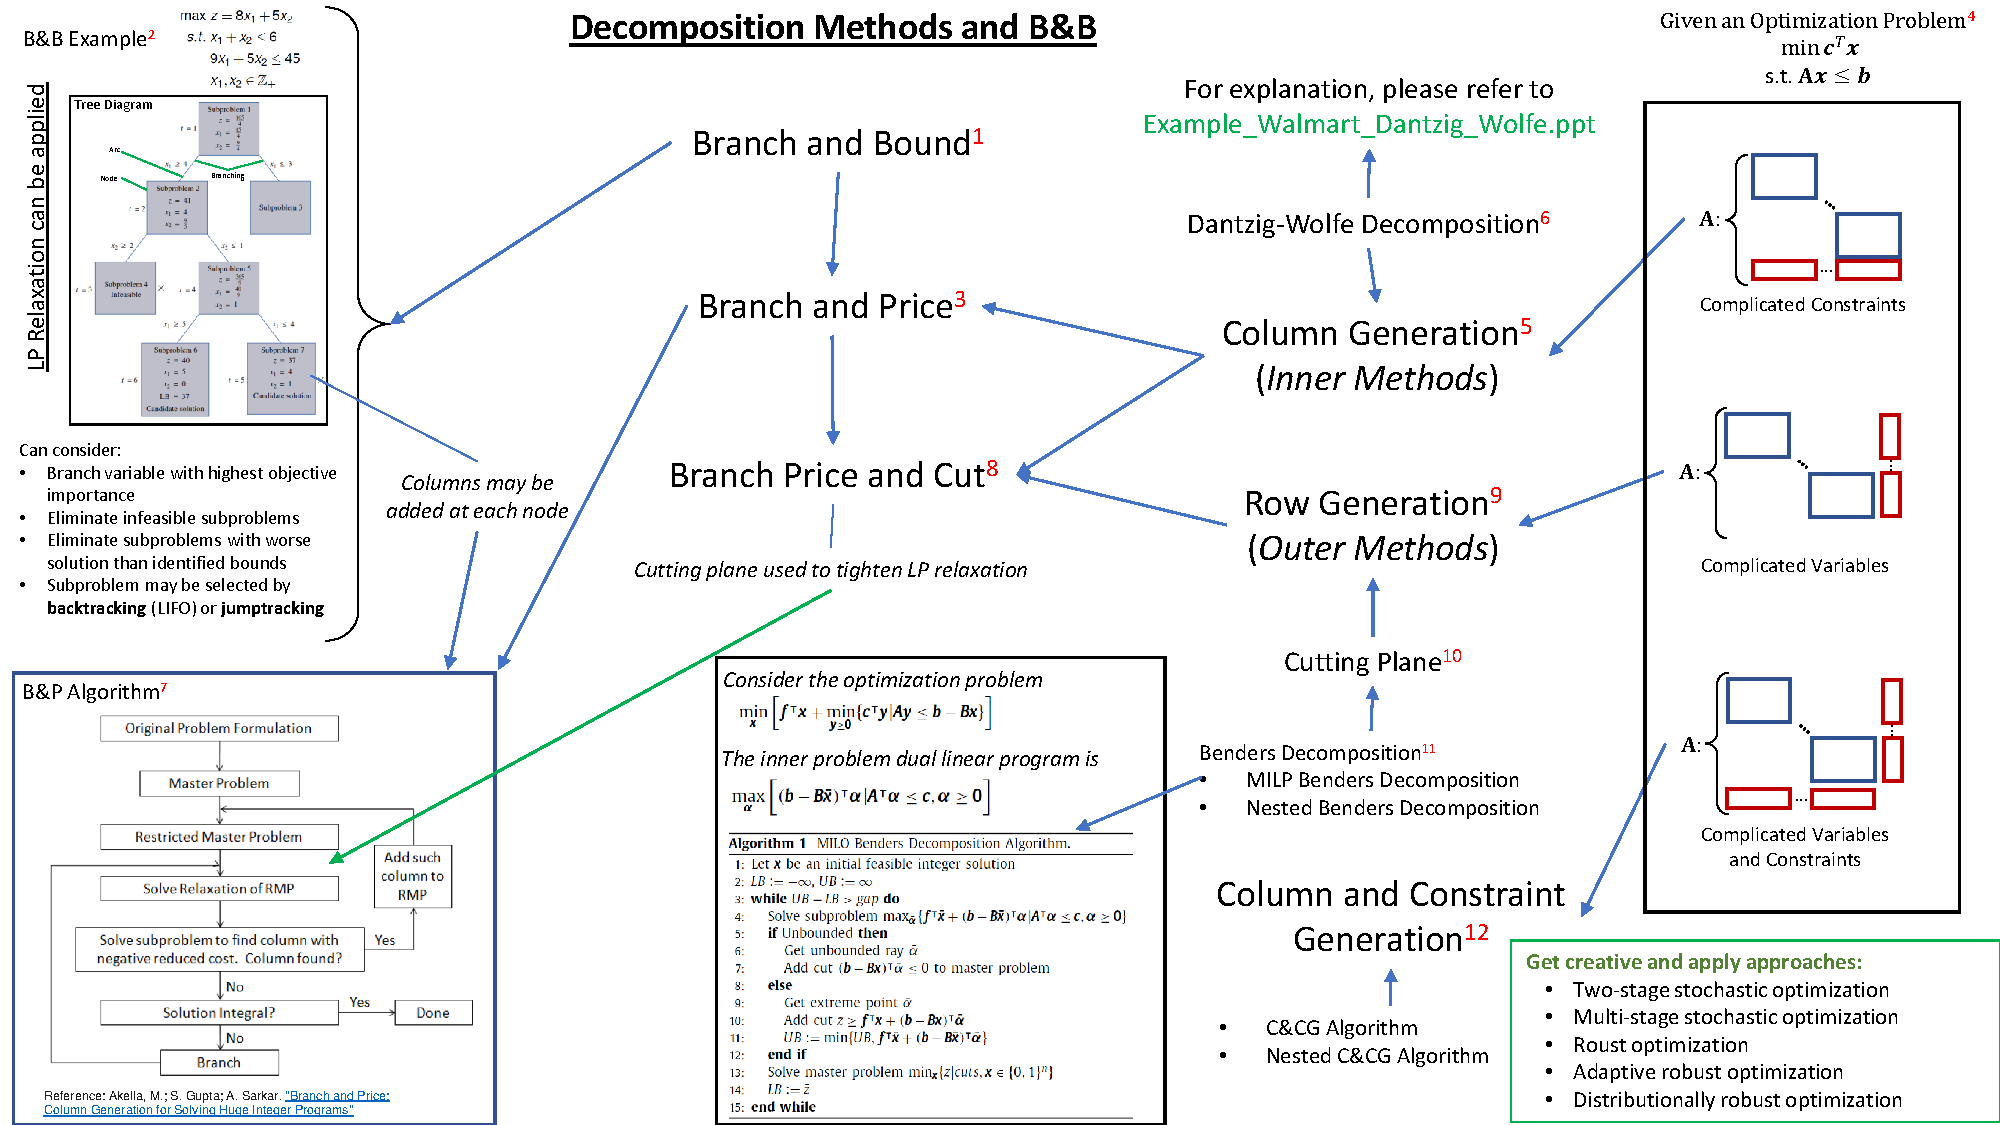
\includegraphics[width = \textwidth]{Decomposition_Techniques_Summary.pdf}
    \label{fig1}
\end{figure}


\newpage
%------------------------------------------------------------------------------------------------------------------------------------
%------------------------------------------------------------------------------------------------------------------------------------
\section{Sorting Problems}\label{section5}

\subsection{IP Sorting Formulation} \label{section5.1}
IP formulation. Therefore, given an array $C$ with elements $c_i, i = 1,\ldots,|C|$, consider the following:\\

\noindent Sets and indices
\begin{itemize}
  \item $I$:~Set of numbers to be sorted, indexed by $i,j$.
\end{itemize}
Parameters
\begin{itemize}
    \item $c_{j}$:~ Value of the $j$ number, i.e., sorting parameter.
\end{itemize}
Variables
\begin{itemize}
  \item $x_{ij}$:~Binary variables that is 1 if $i$ value is assigned $j$ place and 0 otherwise.
\end{itemize}

The IP sorting formulation is presented as follows:

\begin{subequations}
    \begin{align}
    \max_{\pmb{x}}~& \sum_{i \in I} \sum_{i \in J} x_{ij} \tag{Maximize the sum of $x_{ij}$ will determine the sorted array}\\
    \text{s.t. } &  \sum_{j \in I} x_{ij} = 1,~\forall i, \in I \tag{Sorted array elements can only be equal to one of original array}\\
                 & \sum_{i \in I} x_{ji} = 1,~\forall j, \in I \tag{Original array elements can only be equal to one of the sorted array}\\
                 & \sum_{j \in I} c_j x_{ij} \leq  \sum_{j \in I} c_j x_{1+1, j} ,~\forall i, \in I \tag{Sorting restriction}\\
                 & x_{ij} \in \{0,1\}, \forall i, j \in I  \tag{Domain}
    \end{align}
\end{subequations}


\noindent Reference:\\
- Coded by - Daniel Zuniga

\newpage
\subsection{Sorting Algorithms} \label{section5.2}
The following sorting algorithm examples are coded in {\color{blue}\textbf{C++}}.

\noindent Reference:\\
- Coded by - Daniel Zuniga

\subsubsection{Quick sort algorithm} \label{section5.2.2}
Recursively divides the array into two subarrays and assign values depending if each value is greater or smaller than a selected pivot (first or last value of the array cell that is divided).

Performance:
\begin{itemize}
  \item Best $O(n log n)$ - Worst $O(n^2)$, depends on the pivot size.
  \item Auxiliary space $O(n)$.
\end{itemize}

\subsubsection{Merge sort algorithm} \label{section5.2.3}
Iteratively divides the array in two subarrays until single value arrays are defined and merges them in a sorted order.\\

Performance:
\begin{itemize}
  \item Worst $O(n log n)$.
  \item Auxiliary space $O(n)$.
\end{itemize}

\subsubsection{Bubble sort algorithm (recursive)} \label{section5.2.4}
In each iteration, each pair of the array is compared and swapped if it is in the wrong order.\\

Performance:
\begin{itemize}
  \item Best $O(n)$ - Worst $O(n^2)$, depending on the initial arrangement of the values (worst case for reversed sorted).
  \item Auxiliary space $O(1)$ - $O(n)$ for recursive version.
\end{itemize}

\subsubsection{Selection sort algorithm} \label{section5.2.5}
Divides the array into two subsets (sorted and unsorted). Initial sorted subset is empty. In each iteration, the smallest number is identified and assigned to the sorted subset.\\

Performance:
\begin{itemize}
  \item $O(n^2)$
  \item Auxiliary space $O(n)$ for recursive version.
\end{itemize}

\subsubsection{Insertion sort algorithm} \label{section5.2.6}
Divides the array into two subsets (sorted and unsorted),  where the first number ($i=0$) of the array assign to the sorted and the rest to the unsorted. Each iteration assigns the $i+1$ value of the array from the unsorted into the sorted subset in its sorted location.\\

Performance:
\begin{itemize}
  \item Best $O(n)$ - Worst $O(n^2)$, depending on the initial arrangement of the values (worst case for reversed sorted).
  \item Auxiliary space $O(1)$ - $O(n)$ for the recursive version.
\end{itemize}

\newpage
%------------------------------------------------------------------------------------------------------------------------------------
%------------------------------------------------------------------------------------------------------------------------------------
\section{Metaheuristics}\label{section6}

\subsection{Simulated Annealing}\label{section6.1}
Simulated Annealing is coded in {\color{blue}\textbf{Java}} based on the following pseudocode and applied to the Traveling Salesman Problem (TSP) as an illustrative example.

\begin{algorithm}[H]
\SetAlgoLined
\KwResult{Return $x$ as the best solution}
 $h(.)$ is the function to optimize\;
 Generate an initial Temperature $T > 0$ \;
 \While{$T >$ desired $T$}{
    Sample from a symmetrical distribution, e.g., uniform or normal\;
    Add noise to create new candidate solution $x' = x + noise$\;
    Calculate probability $p = exp(\Delta h/T_i)$, where $\Delta h$ is the difference between solutions from $x$ and $x'$\;
    Accept of reject candidate solution with probability $p$; $u \sim U(0,1)$ accept $x = x'$ if $u \leq p$\;
    Update temperature (cooling), e.g., $T = \alpha T$, where $0 < \alpha < 1$
 }
 \caption{Simulated Annealing pseudocode}
\end{algorithm}

\noindent Reference:\\
- Coded by - Daniel Zuniga

\subsection{Tabu Search}\label{section6.2}
Tabu Search is coded in {\color{blue}\textbf{Java}} based on the following pseudocode and applied to the Traveling Salesman Problem (TSP) as an illustrative example.

\begin{algorithm}[H]
\SetAlgoLined
\KwResult{Return $x_o$ as the best solution}
 Set tabu list to null, set $x_o$\;
 \For{ No. Iterations }{
  \{$x_1, x_2,\ldots,x_n$\} = Generate neighborhood $(x_o)$\;
      \For{$i=1, i<=n$}{
        \If{$x_i$ not in tabu list and solution $x_i < x_o$}{
           replace $x_o = x_i$ and\;
           update tabu list:\;
           - add $i$ to tabu list\;
           - decrease tabu list\;
           }
      }
  }
 \caption{Tabu Search pseudocode}
\end{algorithm}


\noindent Reference:\\
- Coded by - Daniel Zuniga

\newpage
\subsection{Particle Swarm Optimization}\label{section6.3}
Particle Swarm Optimization is coded in {\color{blue}\textbf{Java}} based on the following pseudocode and applied to the Traveling Salesman Problem (TSP) as an illustrative example.

\begin{algorithm}[H]
\SetAlgoLined
\KwResult{Return $x_o$ as the best solution}
 Initialize particle list, locations, velocities and solutions $x_{oi}$\;
 Set tabu list to null, set $x$\;
 \For{ No. iterations }{
    \For{ $i = 1$; $i <=$ No. particles }{
        Determine neighbors of particle $i$\;
        \For{ $j = 1$ ; $j <=$ No. neighbor iterations }{
            Determine solution $x_{ij}$ \;
            \If{$x_{ij} < x_{oi}$}{
                $x_{oi} = x_{ij}$\;
            }
        }
        $Sort(x_{oi})$\;
        \If{$x_{o1} < x_o$}{
            Update best solution\;
            $x_o = x_{o1}$\;
        }
    }
    \For{ $i = 1$; $i <=$ No. particles }{
        \For{ $k = 1$; $k <=$ No. locations }{
            Find particle with best solution $x_{oi}$\;
            Select a random vector $rand$ for particle velocity \;
            Update velocity $v_{ik}$ constriction\;
            Update location $l_{ik}$ constriction\;
        }
    }
 }

 \caption{Particle Swarm Optimization pseudocode}
\end{algorithm}

\noindent Reference:\\
- Coded by - Daniel Zuniga
\newpage
\subsection{External Libraries}\label{section6.4}

\subsubsection{OR-Tools - Tabu Search and Simulated Annealing}\label{section6.4.1}
A Vehicle Routing Problem (VRP) is presented using {\color{blue}\textbf{OR-Tools}} and considering two metaheuristic searches are selected to escape local optimum, Tabu Search and Simulated Annealing. The VRP is coded in {\color{blue}\textbf{C++}}.\\

%------------------------------------------------------------------------------------------------------------------------------------
%------------------------------------------------------------------------------------------------------------------------------------
\textbf{Problem Formulation.}
 The goal is to find optimal routes for multiple vehicles visiting a set of destinations, i.e., minimize the total distance from all vehicles.\\

 \noindent - Capacity constraints: vehicles have a maximum distance that can travel.\\
 - Solution limit: iterations before search stops.\\
 - Time limit: time before stopping the search\\
%------------------------------------------------------------------------------------------------------------------------------------
%------------------------------------------------------------------------------------------------------------------------------------

\textbf{Numerical Experiments.}
For the numerical experiment, the parameters are determined as follows:\\

- Distance matrix between all destinations:

\begin{table}[!htbp]	
{\tiny															
    \begin{tabular}{ l l l l l l l l l l l l l l l l l}	
            \{\{0,&   658,    &931,    &835,    &698,    &329,    &602,    &233,    &370,    &233,    &643,    &602,    &466,    &425,    &562,    &931,    &794 \}, \\
            \{658,&   0,      &821,    &370,    &233,    &602,    &876,    &425,    &835,    &890,    &1301,   &713,    &576,    &809,    &1219,   &1042,   &1452\}, \\
            \{931,&   821,    &0,      &1190,   &1054,   &602,    &329,    &972,    &562,    &890,    &480,    &1534,   &1397,   &1356,   &946,    &1862,   &905 \}, \\
            \{835,&   370,    &1190,   &0,      &137,    &780,    &1054,   &602,    &1013,   &1068,   &1478,   &617,    &754,    &986,    &1397,   &672,    &1630\}, \\
            \{698,&   233,    &1054,   &137,    &0,      &643,    &917,    &466,    &876,    &931,    &1342,   &480,    &617,    &850,    &1260,   &809,    &1493\}, \\
            \{329,&   602,    &602,    &780,    &643,    &0,      &274,    &370,    &233,    &288,    &698,    &931,    &794,    &754,    &617,    &1260,   &850 \}, \\
            \{602,&   876,    &329,    &1054,   &917,    &274,    &0,      &643,    &233,    &562,    &425,    &1205,   &1068,   &1027,   &617,    &1534,   &576 \}, \\
            \{233,&   425,    &972,    &602,    &466,    &370,    &643,    &0,      &410,    &466,    &876,    &562,    &425,    &384,    &794,    &890,    &1027\}, \\
            \{370,&   835,    &562,    &1013,   &876,    &233,    &233,    &410,    &0,      &329,    &466,    &972,    &835,    &794,    &384,    &1301,   &617 \}, \\
            \{233,&   890,    &890,    &1068,   &931,    &288,    &562,    &466,    &329,    &0,      &410,    &643,    &506,    &466,    &329,    &972,    &562 \}, \\
            \{643,&   1301,   &480,    &1478,   &1342,   &698,    &425,    &876,    &466,    &410,    &0,      &1054,   &917,    &876,    &466,    &1382,   &425 \}, \\
            \{602,&   713,    &1534,   &617,    &480,    &931,    &1205,   &562,    &972,    &643,    &1054,   &0,      &137,    &370,    &780,    &329,    &1013\}, \\
            \{466,&   576,    &1397,   &754,    &617,    &794,    &1068,   &425,    &835,    &506,    &917,    &137,    &0,      &233,    &643,    &466,    &876 \}, \\
            \{425,&   809,    &1356,   &986,    &850,    &754,    &1027,   &384,    &794,    &466,    &876,    &370,    &233,    &0,      &410,    &506,    &643 \}, \\
            \{562,&   1219,   &946,    &1397,   &1260,   &617,    &617,    &794,    &384,    &329,    &466,    &780,    &643,    &410,    &0,      &917,    &233 \}, \\
            \{931,&   1042,   &1862,   &672,    &809,    &1260,   &1534,   &890,    &1301,   &972,    &1382,   &329,    &466,    &506,    &917,    &0,      &958 \}, \\
            \{794,&   1452,   &905,    &1630,   &1493,   &850,    &576,    &1027,   &617,    &562,    &425,    &1013,   &876,    &643,    &233,    &958,    &0   \},\}\\ 						
    \end{tabular}
    }			
\end{table}	

\noindent - Vehicle available: 4 \\
- Maximum distance per vehicle: 3,000 \\
- Solution limit: 30 \\
- Time limit: 150 seconds\\

\noindent Reference:\\
- Ortools, available at: {\color{blue}https://developers.google.com/optimization}\\
- Coded by - Daniel Zuniga

\newpage
%------------------------------------------------------------------------------------------------------------------------------------
%------------------------------------------------------------------------------------------------------------------------------------
\section{Dynamic Programming and Other Examples}\label{section7}

\subsection{0-1 Knapsack Problem}\label{Section7.1}
The following example is coded in {\color{blue}\textbf{C++}}.\\

There are different kind of items with a weight and value associated and a weight limitation to the bag. The objective is to maximize the value of the objects in the bag.\\

This model has an exponential running time $O(2^n)$. Please refer to 0-1 Knapsack Problem - Dynamic Programming \ref{section5} to increase the computational performance.\\

\noindent Sets and indices
\begin{itemize}
  \item $\mathcal{I}$:~Set of items,indexed by $s$.
\end{itemize}
Parameters
\begin{itemize}
    \item $v_i$:~Value of product $i$. (\$)
    \item $w_i$:~Weight of product $i$. (kg)
    \item $W$:~Weight limit of the bag. (kg)
\end{itemize}
Variables
\begin{itemize}
  \item $x_i$:~Binary variables that is 1 if product $i$ is selected for the bag and 0 otherwise.
\end{itemize}

\begin{subequations}\label{KP}
    \begin{align}
    \max_{\pmb{x}} ~& \sum_{i \in \mathcal{I}} v_i x_i \label{KP1}\\
    \text{s.t. } & \sum_{i \in \mathcal{I}} w_i x_i \leq W \label{KP2}\\
                 & x_i \in \{0,1\},~\forall i \label{KP3}
    \end{align}
\end{subequations}

Objective \eqref{KP1}. Ensures that the weight does not exceed the bag limit \eqref{KP2}; domains \eqref{KP3}.\\

Numerical experiments with the a weight limit $W=50$ and the following products, weights, and values:
\begin{table}[!htbp]
    \centering
    \begin{tabular}{c | c c c c c }
                     & Product 1 & Product 2 & Product 3 & Product 4 & Product 5\\ \hline
        Weight $w_i$ & 12 & 32 & 33 & 5 & 34\\
        Value $v_i$ & 100 & 200 & 50 & 60 & 150
    \end{tabular}
\end{table}

\noindent Reference:\\
- Model - CodesDope, Knapsack Problem, available at: {\color{blue}https://www.codesdope.com/course/algorithms-knapsack-problem/}\\
- Coded by - Daniel Zuniga

\newpage
\subsection{0-1 Knapsack Problem - Dynamic Programming}\label{Section7.2}
The following example is coded in {\color{blue}\textbf{C++}}.\\

There are different kind of items with a weight and value associated and a weight limitation to the bag. The objective is to maximize the value of the objects in the bag.\\

\noindent Sets and indices
\begin{itemize}
  \item $\mathcal{I}$:~Set of items,indexed by $s$.
  \item $\mathcal{W}$:~Set of remaining weights available,indexed by $w$, $W = |\mathcal{W}|$.
\end{itemize}
Parameters
\begin{itemize}
    \item $v_i$:~Value of product $i$. (\$)
    \item $w_i$:~Weight of product $i$. (kg)
    \item $W$:~Weight limit of the bag. (kg)
\end{itemize}
Variable
\begin{itemize}
    \item $CostArray_{i,w}$:~Matrix to store the solution of the function $F(i,w)$.\\
\end{itemize}


Given a function $F(i,w)$ that optimizes the value for the first $i$ products and counter index $w$ for weight limit $W$:

\begin{subequations}\label{KPDP}
    \begin{align}
    & F(i,w) =
    \begin{cases}
        \vspace{0.2cm} F(i-1,w), \text{ if } w_i > w\\
        \vspace{0.2cm} \max\{F(i-1,w),(F(i-1,w-w_i)+v_i)\}, \text{ if } w_i \leq w
    \end{cases} \label{KPDP1}
    \end{align}
\end{subequations}

Dynamic programming function for 0-1 Knapsack problem \eqref{KPDP1}.\\

Numerical experiments with the a weight limit $W=5$ and the following products, weights, and values:
\begin{table}[!htbp]
    \centering
    \begin{tabular}{c | c c c c c}
            & Dummy Product & Product 1 & Product 2 & Product 3 & Product 4 \\ \hline
        Weight $w_i$ & 0 & 3 & 2 & 4 & 1\\
        Value $v_i$ & 0 & 8 & 3 & 9 & 6
    \end{tabular}
\end{table}

\noindent Reference:\\
- Model - CodesDope, Knapsack Problem, available at: {\color{blue}https://www.codesdope.com/course/algorithms-knapsack-problem/}\\
- Coded by - Daniel Zuniga

\newpage
\subsection{Rope Cutting - Dynamic Programming}\label{Section7.3}
The following example is coded in {\color{blue}\textbf{C++}}.\\

Given a rope of size $n$ and a certain number of cuts $c$ of different lengths $l_c$ and sale prices $p_c$, maximize the revenue.\\

\noindent Sets and indices
\begin{itemize}
  \item $\mathcal{C}$:~Set of rope cuts available, indexed by $c$.
  \item $\mathcal{N}$:~Set of remaining rope lengths, indexed by $n$, $N = |\mathcal{N}|$.
\end{itemize}
Parameters
\begin{itemize}
    \item $l_c$:~Length of cut $c$. (m)
    \item $p_c$:~Sale price of cut $c$. (\$)
    \item $N$:~Total length of rope $i$. (m)
\end{itemize}
Variable
\begin{itemize}
    \item $r_n$:~Variable to store the revenue solution.\\
\end{itemize}

The maximize the income, the dynamic approach will be to sell the first cut $p_c$ with $c = n$ and optimize the revenue for the remaining length $r_{N-n}$ as follows:

\begin{equation}\label{RCDP}
    r_N = \max_{1 \leq n \leq N} \{p_n + r_{N-n}\}
\end{equation}

Dynamic programming function for rope cutting problem \eqref{RCDP}.\\

Numerical experiments with a rope length $n=5$ and the following length cuts $l_c$ and sale price per cut $p_c$:
\begin{table}[!htbp]
    \centering
    \begin{tabular}{c | c c c c c c}
            & Dummy Cut & Cut 1 & Cut 2 & Cut 3 & Cut 4 & Cut 5 \\ \hline
        Length $l_c$ (m) & 0 & 1 & 2 & 3 & 4 & 5 \\
        Price $p_c$ (\$) & 0 & 10 & 24 & 30 & 40 & 45
    \end{tabular}
\end{table}

\noindent Reference:\\
- Model - CodesDope, Rod Cutting, available at: {\color{blue}https://www.codesdope.com/course/algorithms-rod-cutting/}\\
- Coded by - Daniel Zuniga

\newpage
\subsection{Coin Change - Dynamic Programming}\label{Section7.4}
The following example is coded in {\color{blue}\textbf{C++}}.\\

Given an amount to sum $A$ and a set of coins  $C$ with their respective values $v_c$, minimize the number of coins to be used.\\

\noindent Sets and indices
\begin{itemize}
  \item $\mathcal{C}$:~Set of coin, indexed by $c$.
  \item $\mathcal{N}$:~Set of remaining sum to be achieved, indexed by $n$, $N = |\mathcal{N}|$.
\end{itemize}
Parameters
\begin{itemize}
    \item $v_c$:~Value of coin $c$. (\$)
    \item $A$:~Amount to sum with coins. (\$)
\end{itemize}
Variable
\begin{itemize}
    \item $n_c$:~Variable to store the number of coins $c$.\\
\end{itemize}

Given a function $M_n$ that minimizes the number of coins $c$ to be used:

\begin{subequations}\label{CCDP}
    \begin{align}
    & M_n =
    \begin{cases}
        \vspace{0.2cm} \min_{c:v_c\leq A} \{M_{n-v_c} + 1\}, \text{ if } n > 0\\
        \vspace{0.2cm} 0, \text{ if } n = 0
    \end{cases} \label{CCDP1}
    \end{align}
\end{subequations}

Dynamic programming function for coin change problem \eqref{CCDP1}.\\

Numerical experiments with an amount to sum of $A=38$ and the following coins $c$ and coin values $v_c$:
\begin{table}[!htbp]
    \centering
    \begin{tabular}{c | c c c c c}
            & Dummy Coin & Coin 1 & Coin 2 & Coin 3 & Coin 4\\ \hline
        Coin value $v_c$ (\$) & 0 & 1 & 2 & 5 & 10
    \end{tabular}
\end{table}


\noindent Reference:\\
- Model - CodesDope, Coin Change, available at: {\color{blue}https://www.codesdope.com/course/algorithms-coin-change/}\\
- Coded by - Daniel Zuniga

\newpage
\subsection{Shortest Path - Dijkstra's - Dynamic Programming}\label{Section7.5}
The following example is coded in {\color{blue}\textbf{C++}}.\\

Given a direct graph $G = (N,E)$ with edge (or arc) length (or length) $d_{ij} \geq 0$ for edge $(i,j) \in E$, identifies the shortest path from the source node (initial) $s$ to the sink node (destination) $t$.\\

\noindent Sets and indices
\begin{itemize}
  \item $\mathcal{N}$:~Set of nodes (or vertex), indexed by $n$.
  \item $\mathcal{E}$:~Set of edges (or links, arcs), indexed by $e$ or $\{ij\}$.
\end{itemize}
Parameters
\begin{itemize}
    \item $d_{ij}$:~Distance from node $i$ to node $j$. (m)
    \item $s$:~Source node (initial)
    \item $t$:~Sink node (destination)
\end{itemize}
Variable
\begin{itemize}
    \item $x_{ij}$:~Binary variable that is 1 is edge between node $i$ and $j$ is selected.
\end{itemize}

\begin{subequations}\label{SP}
    \begin{align}
    \max_{\pmb{x}} ~& \sum_{i,j \in \mathcal{E}} d_{ij} x_{ij} \label{SP1}\\
    \text{s.t. } & \sum_{j:(i,j)\in E} x){ij} - \sum_{j:(j,i) \in E} x_{ji} =
                \begin{cases}
                    \vspace{0.2cm} 1, &\text{ if } i = s\\
                    \vspace{0.2cm} 0, &\forall i \in E \setminus \{s,t\}\\
                    \vspace{0.2cm} -1, &\text{ if } i = t
                \end{cases} \label{SP2}\\
                 & x_{ij} \in \{0,1\},~\forall (i,j) \in E \label{SP3}
    \end{align}
\end{subequations}

Shortest path problem general formulation \eqref{SP}; objective \eqref{SP1}; constraint that sums the edges of all paths \eqref{SP2}; domains \eqref{SP3}.

\newpage
Numerical experiments with ten nodes, $N = 10$, twenty edges, $E = 20$, five decision making stages $S=5$ (initial node $s=1$, destination $s=5$), and the following distance matrix $c_{ij}$:
\begin{table}[!htbp]
    \centering
    \begin{tabular}{c c | c c c c c c c c c c}\\
	&		&	\multicolumn{10}{c}{j}	\\																		
	&	$c_{ij}$	&	1	&	2	&	3	&	4	&	5	&	6	&	7	&	8	&	9	&	10	\\ \hline
\multirow{10}{*}{i}	&	1	&	0	&	550	&	900	&	770	&	0	&	0	&	0	&	0	&	0	&	0	\\
	&	2	&	550	&	0	&	0	&	0	&	680	&	790	&	1050	&	0	&	0	&	0	\\
	&	3	&	900	&	0	&	0	&	0	&	580	&	760	&	700	&	0	&	0	&	0	\\
	&	4	&	770	&	0	&	0	&	0	&	510	&	700	&	830	&	0	&	0	&	0	\\
	&	5	&	0	&	680	&	580	&	510	&	0	&	0	&	0	&	610	&	790	&	0	\\
	&	6	&	0	&	790	&	760	&	700	&	0	&	0	&	0	&	540	&	940	&	0	\\
	&	7	&	0	&	1050	&	700	&	830	&	0	&	0	&	0	&	790	&	270	&	0	\\
	&	8	&	0	&	0	&	0	&	0	&	610	&	540	&	790	&	0	&	0	&	1030	\\
	&	9	&	0	&	0	&	0	&	0	&	790	&	940	&	270	&	0	&	0	&	1390	\\
	&	10	&	0	&	0	&	0	&	0	&	0	&	0	&	0	&	1030	&	1390	&	0	\\
    \end{tabular}
\end{table}

\begin{figure}[!htbp]or
    \centering
    \includegraphics[width = 0.4\textwidth]{Shortest_Path_Dijsktra.PNG}
\end{figure}

\noindent Reference:\\
- Coded by - Daniel Zuniga

\newpage
\subsection{Minimum Dominating Set}\label{Section7.6}
The following example is coded in {\color{blue}\textbf{C++}}.\\

\pmb{Minimum dominating set} (MDS) problem: given an (undirected) graph $G = (V,E)$ with vertex set $V$ and edge set $E$, where $V$ has $n$ vertices, and $E$ is expressed by adjacency matrix $A = (a_{ij})_{n*n}$ such that $a_{ij}=1$ if there is an edge between $i$ and $j (i \neq j)$, and $a_{ii} = 0$. The problem is to find a subset $D \subseteq V$ with smallest cardinality such that every vertex of $V$ is either chosen into the subset $D$ or has at least one neighbor in $D$.\\

$x_i \in \{0,1\}$: a binary variable indicates that whether vertex $i$ is chosen into $D$ if $x_i=1$ or not if $x_i=0$

\begin{subequations}\label{MDS}
    \begin{align}
    \min_{\pmb{x}} ~& \sum_{i =1}^n x_i \label{MDS1}\\
    \text{s.t. } & x_i + \sum_{j = 1, j \neq i}^n a_{ij} x_j \geq 1,~ \forall i \in V \label{MDS2}\\
                 & x_i \in \{0,1\}, \forall i \in V \label{MDS3}
    \end{align}
\end{subequations}

Objective \eqref{MDS1}. Minimum dominating set constraint \eqref{MDS2}; domains \eqref{MDS3}.\\

Numerical experiments with $V = 14$ vertex or nodes and $E = 20$ edges or vertices.
\begin{table}[!htbp]
    \centering
    \begin{tabular}{c | c c c c c c c c c c c c c c c c c c c c}
        Edge No   & 1 & 2 & 3 & 4 & 5 & 6 & 7 & 8 & 9 & 10 & 11& 12& 13& 14 & 15 & 16& 17& 18 & 19 & 20\\ \hline
        From Node & 2 & 5 & 3 & 4 & 5 & 4 & 5 & 7 & 9 & 6 & 11& 12& 13& 8 & 9 & 10& 14& 11 & 14 & 14\\
        To Node   & 1 & 1 & 2 & 2 & 2 & 3 & 4 & 4 & 4 & 5 & 6 & 6 & 6 & 7 & 7 & 9 & 9 & 10 & 12 & 13
    \end{tabular}
\end{table}

\noindent Reference:\\
- Coded by - Daniel Zuniga

\newpage
\subsection{Optimum Assignment Problem}\label{Section7.7}
The following example is coded in {\color{blue}\textbf{C++}}.\\

Identify the job assignment that will maximize the production.

\noindent Sets and indices
\begin{itemize}
  \item $\mathcal{I}$:~Set of production factories,indexed by $s$.
  \item $\mathcal{J}$:~Set of products, indexed by $j$.
\end{itemize}
Parameters
\begin{itemize}
    \item $a_{ij}$:~Production rate of product $j$ at factory $i$. (products/time)
\end{itemize}
Variables
\begin{itemize}
  \item $x_{ij}$:~Binary variables that is 1 if factory $i$ is assigned product $j$ and 0 otherwise.
\end{itemize}

\begin{subequations}\label{OJA}
    \begin{align}
    \max_{\pmb{x}} ~& \sum_{i \in \mathcal{I}} \sum_{j \in \mathcal{J}} a_{ij} x_{ij} \label{OJA1}\\
    \text{s.t. } & \sum_{j \in \mathcal{J}} x_{ij} = 1,~ \forall i \label{OJA2}\\
                 & \sum_{i \in \mathcal{I}} x_{ij} = 1,~ \forall j \label{OJA3}\\
                 & x_{ij} \in \{0,1\},~\forall i, \forall j \label{OJA4}
    \end{align}
\end{subequations}

Objective \eqref{OJA1}. Constraints are as follows: each factory $i$ can only produce one product $j$ \eqref{OJA2}; each product $j$ can only be assigned to one factory $i$ \eqref{OJA3}; domains \eqref{OJA4}.\\

Numerical experiments with the following factories, products, and production rates:
\begin{table}[!htbp]
    \centering
    \begin{tabular}{c | c c c c c }
        Factory & Product 1 & Product 2 & Product 3 & Product 4 & Product 5\\ \hline
        Factory 1 & 12 & 6 & 8 & 7 & 8\\
        Factory 2 & 6 & 8 & 7 & 10 & 3\\
        Factory 3 & 8 & 11 & 12 & 5 & 9\\
        Factory 4 & 9 & 12 & 6 & 11 & 15\\
        Factory 5 & 10 & 7 & 12 & 9 & 7
    \end{tabular}
\end{table}

\noindent Reference:\\
- Coded by - Daniel Zuniga

\newpage
%------------------------------------------------------------------------------------------------------------------------------------
%------------------------------------------------------------------------------------------------------------------------------------
\section{SQL}\label{section8}

A SQL example is presented using for {\color{blue}\textbf{Particle Swarm Optimization}}, coded in {\color{blue}\textbf{Java}}, and using {\color{blue}\textbf{MySQL}}.
\end{document}
